\documentclass[12pt, answers]{exam}
%\documentclass[12pt]{exam}
\usepackage[utf8]{inputenc}
\usepackage{soul}
\usepackage{bm}
\usepackage{listings}
\usepackage{pgfplots} 
\pgfplotsset{compat=newest}
\usepackage[marginparsep=16pt, margin=1.75in, showframe]{geometry}
%\usepackage[marginparsep=16pt, margin=1.0in]{geometry}

\usepackage{amsmath,amssymb}
\usepackage{multicol}
\usepackage{marginnote}

\newcommand{\class}{PHDCW-101}
\newcommand{\term}{2019 Semester}
\newcommand{\examnum}{End-Semester Examination}
\newcommand{\examdate}{\today}
\newcommand{\timelimit}{60 Minutes}


\lstset{
	basicstyle=\ttfamily,
	columns=fullflexible,
	frame=single,
	breaklines=true
}


\pagestyle{head}
\firstpageheader{}{}{}
\runningheader{\class}{\examnum\ - Page \thepage\ of \numpages}{\examdate}
\runningheadrule
\DeclareMathOperator{\sech}{sech}
\begin{document}

\noindent
\begin{tabular*}{\textwidth}{l @{\extracolsep{\fill}} r @{\extracolsep{6pt}} l}
\textbf{\class} & \\
\textbf{\term} &&\\
\textbf{\examnum} &&\\
\textbf{\examdate} &&\\
\textbf{Time Limit: \timelimit} & Instructor: Dr. Analabha Roy
\end{tabular*}\\
\rule[2ex]{\textwidth}{2pt}

\begin{questions}

\question\marginnote{$10$} Answer any $5$ questions.
\begin{parts}
\part\marginnote{$2$}  What will be the output of the following python program?
\begin{lstlisting}[language=Python]
import numpy as np
e  = np.array([[1,2,3], [4,5,6]])
print(e)
print(e.reshape(3,2))
\end{lstlisting}
\part\marginnote{$2$}  Write LaTeX expressions for rendering the following equations.
\begin{subparts}
	\subpart
	\begin{equation}
	\int^\infty_0\mathrm{d}x\;\frac{\sin{x}}{x} = \frac{\pi}{2}.\nonumber
	\end{equation}
	\subpart
	\begin{equation}
	\sum^N_{n=0} r^n = \frac{1-r^N}{1-r}.\nonumber
	\end{equation}
\end{subparts}	
\part\marginnote{$2$} Describe the different types of loop statements in C programs.
\part\marginnote{$2$} What are the criteria for granting a patent? Give two inventions that are not patentable.
\part\marginnote{$2$} Find the inverse $z-$ transform of the function $F(z)=\displaystyle\frac{6}{z-2}$.
\part\marginnote{$2$}  What are the possible types of fixed points in a two dimensional system ?
%\part\marginnote{$2$}What are the different disciplines by which a research can be classified?
%\part\marginnote{$2$}What do you mean by meta search engines? Give examples.
\part\marginnote{$2$}Power in a circuit is measured by measuring a current through a resistor. The current is measured with an accuracy of $\pm 1.5\% $ and the tolerance band of the resistor is $\pm 0.5\%$. The errors are limiting or guarantee errors. Find the accuracy with which the power is measured.
%\part\marginnote{$2$}  What do you mean by precise and accurate measurements? 
\end{parts}

\question\marginnote{$40$}  Answer any $4$ questions.

\begin{parts}
	\part\marginnote{$10$} 
	Write down the output of the following \LaTeX \ snippet.
	\begin{lstlisting}[language=TeX]
	\documentclass [12pt,a4] {article}
	
	\usepackage{amsmath}
	
	\title{{\Large	\bf Chaos in the Quantum Double Well Oscillator:\\The Ehrenfest View Revisited}}
	\begin{document}
	\maketitle
	Pattanayak and Schieve explored the semiquantal dynamics of the double well oscillator governed by the Hamiltonian
	\begin{equation}
	H = \frac{P^2} {2} - \frac{1} {2} \ x^2 + \frac{\lambda} {4} \ x^4
	\end{equation}
	The classical dynamics of this oscillator is obviously regular, as explained in Landau-Lifshitz (Vol. 1), being a periodic trajectory
	centered about $x = \pm \displaystyle\frac{1} {\sqrt{\lambda}}$ for total energy $E$ in the range  $0 > E > -1/4$ and about $x=0$ for $E>0$. It was shown, based on an Ehrenfest equation approach that in the semiquantal limit the quantum fluctuations cause the dynamics of this oscillator to become chaotic with four repelling zones in the phase space.  
	
	The semiquantal  Ehrenfest dynamics of the centroid $\langle x\rangle$ of a wave packet is given by
	\begin{equation}
	\langle \ddot x\rangle = \langle x\rangle - \lambda \langle x^3\rangle ,
	\end{equation}
	\textit{i.e.}
	\begin{equation}
	\langle\ddot x\rangle - \langle x\rangle + \lambda \langle x\rangle^3 
	= \lambda \left[\langle x\rangle^3 - \langle x^3\rangle\right] = Q
	\end{equation}
	With this in mind, the class of quantum wave packets that we
	will work with is
	\begin{equation}
	\psi (x,t) = N_1 (t) e^{- \left(x-a_0 - \epsilon (t)\right)^2/2 b^2_0} + 
	N_2 (t) e^{- \left(x+a_0 + \epsilon (t)\right)^2/2 b^2_0} .
	\end{equation}
	
	Turning to the dynamics, we now have the result
	\begin{subequations}
	\begin{equation}
	\langle x\rangle = (a_0 + \epsilon) (N_1^2 - N_2^2), 
	\end{equation}
	\begin{equation}
	\langle x^3\rangle = (a_0 + \epsilon) \left[(a_0 + \epsilon)^2 
	+ \frac{3} {2} b^2_0\right] (N_1^2 - N^2_2) .
	\end{equation}
	\end{subequations}
	\end{document}
	\end{lstlisting}
	\pagebreak
\part\marginnote{$10$}  Answer the following questions.
\begin{subparts}
	\subpart\marginnote{$4$}  Name and describe four interfaces to the Unix/Linux kernel.
	\subpart\marginnote{$4$}  Briefly describe the four stages of the building processes of a C program.
	\subpart\marginnote{$2$}  What are the differences between a high-level and mid-level programming language?
\end{subparts}	
\part\marginnote{$10$}  Answer the following questions:
\begin{subparts}
    \subpart\marginnote{$2$}What are functions in the C programming language? 
    \subpart\marginnote{$4$}What are the different ways of writing functions in C programs? 
    \subpart\marginnote{$4$}Write a program in C to find the factorial of an integer using a recursive function.
\end{subparts}
\part\marginnote{$10$}  Answer the following questions.
\begin{subparts}
	\subpart\marginnote{$5$}Write down the normal distribution function explaining the symbols therein. Show that $\sigma^2 = \overline{x^2}-\bar{x}^2 $, where the symbols have their usual meaning. 
	\subpart\marginnote{$3$}A box contains $100 \Omega $ resistors which are known to have a standard deviation of $2 \Omega$. What is the probability of finding a resistor in the range $99-101 \;\Omega$ ? 
	\subpart\marginnote{$2$} Consider error propagation through a single-variable function $Z = f(A)$.
	Here, $\alpha_A$ represents the error on the mean $\bar{A}$ . Show that the uncertainty in $Z$ can also be represented as $\alpha_Z = \left|\displaystyle\frac{\mathrm{d}Z}{\mathrm{d}A}\right|\alpha_A$.
\end{subparts}
\part\marginnote{$10$} Answer the following questions.
\addpoints
\begin{subparts}
	\subpart\marginnote{$4$}  What are main motivations for publishing an article in a scientific
	journal?
	\subpart\marginnote{$2$} Give two advantages of e-journals over conventional print journals.	
	\subpart\marginnote{$2$}What do you mean by a ‘DATABASE’? Write at least two different kinds
	of databases available on the internet. 	
	\subpart\marginnote{$2$}What do you mean by open access repositories? Give an example. 
\end{subparts}
\part\marginnote{$10$}  Answer the following questions.
\begin{subparts}
	\subpart\marginnote{$6$} Find the Laplace transform of the rectangular wave given in the figure below:
	\begin{center}
		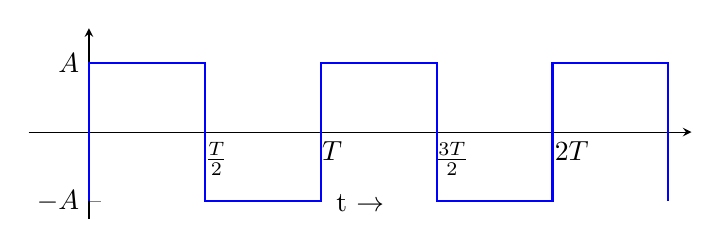
\begin{tikzpicture}
		\begin{axis}[
		width=10cm,
		height=4cm,
		x axis line style={-stealth},
		y axis line style={-stealth},
		xticklabels={$\;\;\;\frac{T}{2}$,$\;\;\;T$, $\;\;\;\;\frac{3T}{2}$, $\;\;\;\;\;2T$}, xtick={1,...,4},
		ymax = 1.5,xmax=5.2,
		axis lines*=center,
		yticklabels={$-A$, $A$}, ytick={-1,1},
		xlabel={t $\rightarrow$},
		xlabel near ticks,
		ylabel near ticks]
		\addplot+[thick,mark=none,const plot]
		coordinates
		{(0,-1) (0,1) (1,-1) (2,1) (3,-1) (4,1) (5,-1)};
		\end{axis}
		\end{tikzpicture}
	\end{center}
	\subpart\marginnote{$4$} Find the eigenvalues and the eigenvectors of the spin operator of an
	electron in an arbitrary direction, specified by the unit vector.
\end{subparts}
\part\marginnote{$10$}  Answer the following questions.
\begin{subparts}
\subpart\marginnote{$6$}  Consider the following pendulum equation: $\ddot{x} + \sin{x}=0 $.
\begin{subsubparts}
\subsubpart\marginnote{$3$} Derive the fixed points and identify the nature of the fixed points. 
\subsubpart\marginnote{$2$} Draw the qualitative phase portrait of the dynamics.
\subsubpart\marginnote{$1$}  Explain the physics of the pendulum from the phase portrait above.
\end{subsubparts}
\subpart\marginnote{$4$}Find the energy eigenvalues of a particle moving in a one dimensional
anharmonic potential $V(x) = Kx^2 + bx^3$, where $K$ and $b$ are constants ($b\ll 1$).  
\end{subparts}
%\part\marginnote{$10$}  Answer the following questions
%\begin{subparts}
%\subpart\marginnote{$4$} Write down the statement of theory of least squares. An observer measures a physical quantity as $1.70, 1.78, 1.74$, $1.79$, and $1.74$. Apply the theory of least squares to find the most probable
%value.
%\subpart\marginnote{$3$} Applying theory of least squares, set up the normal equations for a straight line $y=a+bx$.
%\subpart\marginnote{$3$}Two resistances $100\Omega \pm 5\Omega $ and $150\Omega \pm 15\Omega $ are connected in series. If the deviations are standard deviations, how the resultant resistance can be expressed? 
%\end{subparts}

\end{parts}


\end{questions}

\end{document}